\documentclass[9pt,handout]{beamer}
\setbeamertemplate{caption}[numbered]
\usetheme[white]{Illinois}
%\title[short title]{long title}
\title[HALEU Transitions]{Comparing HALEU Demand Among Advanced Reactor 
Fuel Cycle Transitions}
\author[Amanda M. Bachmann]{Amanda M. Bachmann, Kathryn D. Huff\\Advanced Reactors and Fuel Cycles Group}
%\author[Kathryn D. Huff]{Kathryn D. Huff\\Advanced Reactors and Fuel Cycles Group}
\date[06.16.2021]{June 16, 2021}
\institute[UIUC]{University of Illinois at Urbana-Champaign}

%\usepackage{bbding}
\usepackage{amsfonts}
\usepackage{amsmath}
\usepackage{xspace}
\usepackage{graphicx}
\usepackage{subfigure}
\usepackage{booktabs} % nice rules for tables
\usepackage{microtype} % if using PDF
\usepackage{bigints}
%\usepackage{minted}

\newcommand{\units}[1] {\:\text{#1}}%
\newcommand{\SN}{S$_N$}%{S$_\text{N}$}%{$S_N$}%
\newcommand{\Cyclus}{\textsc{Cyclus}\xspace} %
\newcommand{\Cycamore}{\textsc{Cycamore}\xspace} %
\DeclareMathOperator{\erf}{erf}
%I need some complimentary error funcitons... 
\DeclareMathOperator{\erfc}{erfc}
%Those icons in the references are terrible looking
\setbeamertemplate{bibliography item}[text]

%%%% Acronym support

\usepackage[acronym,toc]{glossaries}
%\newacronym{<++>}{<++>}{<++>}
\newacronym[longplural={metric tons of heavy metal}]{MTHM}{MTHM}{metric ton of heavy metal}
\newacronym{ABM}{ABM}{agent-based modeling}
\newacronym{ACDIS}{ACDIS}{Program in Arms Control \& Domestic and International Security}
\newacronym{AHTR}{AHTR}{Advanced High Temperature Reactor}
\newacronym{ANDRA}{ANDRA}{Agence Nationale pour la gestion des D\'echets RAdioactifs, the French National Agency for Radioactive Waste Management}
\newacronym{ANL}{ANL}{Argonne National Laboratory}
\newacronym{API}{API}{application programming interface}
\newacronym{ARE}{ARE}{Aircraft Reactor Experiment}
\newacronym{ARFC}{ARFC}{Advanced Reactors and Fuel Cycles}
\newacronym{ASME}{ASME}{American Society of Mechanical Engineers}
\newacronym{ATWS}{ATWS}{Anticipated Transient Without Scram}
\newacronym{BDBE}{BDBE}{Beyond Design Basis Event}
\newacronym{BIDS}{BIDS}{Berkeley Institute for Data Science}
\newacronym{CAFCA}{CAFCA}{ Code for Advanced Fuel Cycles Assessment }
\newacronym{CDTN}{CDTN}{Centro de Desenvolvimento da Tecnologia Nuclear}
\newacronym{CEA}{CEA}{Commissariat \`a l'\'Energie Atomique et aux \'Energies Alternatives}
\newacronym{CI}{CI}{continuous integration}
\newacronym{CNEN}{CNEN}{Comiss\~{a}o Nacional de Energia Nuclear}
\newacronym{CNERG}{CNERG}{Computational Nuclear Engineering Research Group}
\newacronym{COSI}{COSI}{Commelini-Sicard}
\newacronym{COTS}{COTS}{commercial, off-the-shelf}
\newacronym{CSNF}{CSNF}{commercial spent nuclear fuel}
\newacronym{CTAH}{CTAHs}{Coiled Tube Air Heaters}
\newacronym{CUBIT}{CUBIT}{CUBIT Geometry and Mesh Generation Toolkit}
\newacronym{CURIE}{CURIE}{Centralized Used Fuel Resource for Information Exchange}
\newacronym{DAG}{DAG}{directed acyclic graph}
\newacronym{DANESS}{DANESS}{Dynamic Analysis of Nuclear Energy System Strategies}
\newacronym{DBE}{DBE}{Design Basis Event}
\newacronym{DESAE}{DESAE}{Dynamic Analysis of Nuclear Energy Systems Strategies}
\newacronym{DHS}{DHS}{Department of Homeland Security}
\newacronym{DOE}{DOE}{Department of Energy}
\newacronym{DRACS}{DRACS}{Direct Reactor Auxiliary Cooling System}
\newacronym{DRE}{DRE}{dynamic resource exchange}
\newacronym{DSNF}{DSNF}{DOE spent nuclear fuel}
\newacronym{DYMOND}{DYMOND}{Dynamic Model of Nuclear Development }
\newacronym{EBS}{EBS}{Engineered Barrier System}
\newacronym{EDZ}{EDZ}{Excavation Disturbed Zone}
\newacronym{EIA}{EIA}{U.S. Energy Information Administration}
\newacronym{EPA}{EPA}{Environmental Protection Agency}
\newacronym{EP}{EP}{Engineering Physics}
\newacronym{FCO}{FCO}{Fuel Cycle Options}
\newacronym{FCT}{FCT}{Fuel Cycle Technology}
\newacronym{FEHM}{FEHM}{Finite Element Heat and Mass Transfer}
\newacronym{FEPs}{FEPs}{Features, Events, and Processes}
\newacronym{FHR}{FHR}{Fluoride-Salt-Cooled High-Temperature Reactor}
\newacronym{FLiBe}{FLiBe}{Fluoride-Lithium-Beryllium}
\newacronym{GDSE}{GDSE}{Generic Disposal System Environment}
\newacronym{GDSM}{GDSM}{Generic Disposal System Model}
\newacronym{GENIUSv1}{GENIUSv1}{Global Evaluation of Nuclear Infrastructure Utilization Scenarios, Version 1}
\newacronym{GENIUSv2}{GENIUSv2}{Global Evaluation of Nuclear Infrastructure Utilization Scenarios, Version 2}
\newacronym{GENIUS}{GENIUS}{Global Evaluation of Nuclear Infrastructure Utilization Scenarios}
\newacronym{GPAM}{GPAM}{Generic Performance Assessment Model}
\newacronym{GRSAC}{GRSAC}{Graphite Reactor Severe Accident Code}
\newacronym{GUI}{GUI}{graphical user interface}
\newacronym{HLW}{HLW}{high level waste}
\newacronym{HPC}{HPC}{high-performance computing}
\newacronym{HTC}{HTC}{high-throughput computing}
\newacronym{HTGR}{HTGR}{High Temperature Gas-Cooled Reactor}
\newacronym{IAEA}{IAEA}{International Atomic Energy Agency}
\newacronym{IEMA}{IEMA}{Illinois Emergency Mangament Agency}
\newacronym{INL}{INL}{Idaho National Laboratory}
\newacronym{IPRR1}{IRP-R1}{Instituto de Pesquisas Radioativas Reator 1}
\newacronym{IRP}{IRP}{Integrated Research Project}
\newacronym{ISFSI}{ISFSI}{Independent Spent Fuel Storage Installation}
\newacronym{ISRG}{ISRG}{Independent Student Research Group}
\newacronym{JFNK}{JFNK}{Jacobian-Free Newton Krylov}
\newacronym{LANL}{LANL}{Los Alamos National Laboratory}
\newacronym{LBNL}{LBNL}{Lawrence Berkeley National Laboratory}
\newacronym{LCOE}{LCOE}{levelized cost of electricity}
\newacronym{LDRD}{LDRD}{laboratory directed research and development}
\newacronym{LFR}{LFR}{Lead-Cooled Fast Reactor}
\newacronym{LLNL}{LLNL}{Lawrence Livermore National Laboratory}
\newacronym{LMFBR}{LMFBR}{Liquid Metal Fast Breeder Reactor}
\newacronym{LOFC}{LOFC}{Loss of Forced Cooling}
\newacronym{LOHS}{LOHS}{Loss of Heat Sink}
\newacronym{LOLA}{LOLA}{Loss of Large Area}
\newacronym{LP}{LP}{linear program}
\newacronym{MA}{MA}{minor actinide}
\newacronym{MCNP}{MCNP}{Monte Carlo N-Particle code}
\newacronym{MILP}{MILP}{mixed-integer linear program}
\newacronym{MIT}{MIT}{the Massachusetts Institute of Technology}
\newacronym{MOAB}{MOAB}{Mesh-Oriented datABase}
\newacronym{MOOSE}{MOOSE}{Multiphysics Object-Oriented Simulation Environment}
\newacronym{MOX}{MOX}{mixed oxide}
\newacronym{MSBR}{MSBR}{Molten Salt Breeder Reactor}
\newacronym{MSRE}{MSRE}{Molten Salt Reactor Experiment}
\newacronym{MSR}{MSR}{Molten Salt Reactor}
\newacronym{NAGRA}{NAGRA}{National Cooperative for the Disposal of Radioactive Waste}
\newacronym{NEAMS}{NEAMS}{Nuclear Engineering Advanced Modeling and Simulation}
\newacronym{NEUP}{NEUP}{Nuclear Energy University Programs}
\newacronym{NFCSim}{NFCSim}{Nuclear Fuel Cycle Simulator}
\newacronym{NGNP}{NGNP}{Next Generation Nuclear Plant}
\newacronym{NMWPC}{NMWPC}{Nuclear MW Per Capita}
\newacronym{NNSA}{NNSA}{National Nuclear Security Administration}
\newacronym{NPRE}{NPRE}{Department of Nuclear, Plasma, and Radiological Engineering}
\newacronym{NQA1}{NQA-1}{Nuclear Quality Assurance - 1}
\newacronym{NRC}{NRC}{Nuclear Regulatory Commission}
\newacronym{NSF}{NSF}{National Science Foundation}
\newacronym{NSSC}{NSSC}{Nuclear Science and Security Consortium}
\newacronym{NUWASTE}{NUWASTE}{Nuclear Waste Assessment System for Technical Evaluation}
\newacronym{NWF}{NWF}{Nuclear Waste Fund}
\newacronym{NWTRB}{NWTRB}{Nuclear Waste Technical Review Board}
\newacronym{OCRWM}{OCRWM}{Office of Civilian Radioactive Waste Management}
\newacronym{ORION}{ORION}{ORION}
\newacronym{ORNL}{ORNL}{Oak Ridge National Laboratory}
\newacronym{PARCS}{PARCS}{Purdue Advanced Reactor Core Simulator}
\newacronym{PBAHTR}{PB-AHTR}{Pebble Bed Advanced High Temperature Reactor}
\newacronym{PBFHR}{PB-FHR}{Pebble-Bed Fluoride-Salt-Cooled High-Temperature Reactor}
\newacronym{PEI}{PEI}{Peak Environmental Impact}
\newacronym{PH}{PRONGHORN}{PRONGHORN}
\newacronym{PRKE}{PRKE}{Point Reactor Kinetics Equations}
\newacronym{PSPG}{PSPG}{Pressure-Stabilizing/Petrov-Galerkin}
\newacronym{PWAR}{PWAR}{Pratt and Whitney Aircraft Reactor}
\newacronym{PWR}{PWR}{Pressurized Water Reactor}
\newacronym{PyNE}{PyNE}{Python toolkit for Nuclear Engineering}
\newacronym{PyRK}{PyRK}{Python for Reactor Kinetics}
\newacronym{QA}{QA}{quality assurance}
\newacronym{RDD}{RD\&D}{Research Development and Demonstration}
\newacronym{RD}{R\&D}{Research and Development}
\newacronym{RELAP}{RELAP}{Reactor Excursion and Leak Analysis Program}
\newacronym{RIA}{RIA}{Reactivity Insertion Accident}
\newacronym{RIF}{RIF}{Region-Institution-Facility}
\newacronym{SFR}{SFR}{Sodium-Cooled Fast Reactor}
\newacronym{SINDAG}{SINDA{\textbackslash}G}{Systems Improved Numerical Differencing Analyzer $\backslash$ Gaski}
\newacronym{SKB}{SKB}{Svensk K\"{a}rnbr\"{a}nslehantering AB}
\newacronym{SNF}{SNF}{spent nuclear fuel}
\newacronym{SNL}{SNL}{Sandia National Laboratory}
\newacronym{STC}{STC}{specific temperature change}
\newacronym{SUPG}{SUPG}{Streamline-Upwind/Petrov-Galerkin}
\newacronym{SWF}{SWF}{Separations and Waste Forms}
\newacronym{SWU}{SWU}{Separative Work Unit}
\newacronym{TRIGA}{TRIGA}{Training Research Isotope General Atomic}
\newacronym{TRISO}{TRISO}{Tristructural Isotropic}
\newacronym{TSM}{TSM}{Total System Model}
\newacronym{TSPA}{TSPA}{Total System Performance Assessment for the Yucca Mountain License Application}
\newacronym{ThOX}{ThOX}{thorium oxide}
\newacronym{UFD}{UFD}{Used Fuel Disposition}
\newacronym{UML}{UML}{Unified Modeling Language}
\newacronym{UOX}{UOX}{uranium oxide}
\newacronym{UQ}{UQ}{uncertainty quantification}
\newacronym{US}{US}{United States}
\newacronym{UW}{UW}{University of Wisconsin}
\newacronym{VISION}{VISION}{the Verifiable Fuel Cycle Simulation Model}
\newacronym{VV}{V\&V}{verification and validation}
\newacronym{WIPP}{WIPP}{Waste Isolation Pilot Plant}
\newacronym{YMR}{YMR}{Yucca Mountain Repository Site}


\usepackage{tikz}
\usetikzlibrary{shapes.geometric, arrows}
\usetikzlibrary{positioning, arrows, decorations, shapes}

\tikzstyle{agent} = [rectangle, rounded corners, minimum width=0.1cm, minimum height=0.2cm,text centered, draw=black, fill=blue!30]
\tikzstyle{transition} = [rectangle, rounded corners, minimum width=0.1cm, minimum height=0.2cm,text centered, draw=black, fill=red!30]
\tikzstyle{arrow} = [thick,->,>=stealth]

\tikzstyle{region} = [rectangle, rounded corners, minimum width=0.1cm, minimum height=0.2cm,text centered, draw=black, fill=green!30]
\tikzstyle{institution} = [rectangle, rounded corners, minimum width=0.1cm, minimum height=0.2cm,text centered, draw=black, fill=red!30]
\tikzstyle{facility} = [rectangle, rounded corners, minimum width=0.1cm, minimum height=0.2cm,text centered, draw=black, fill=blue!30]
\tikzstyle{connect} = [thick,-]
\makeglossaries

%try to get rid of header on title page\dots
\makeatletter
    \newenvironment{withoutheadline}{
        \setbeamertemplate{headline}[default]
        \def\beamer@entrycode{\vspace*{-\headheight}}
    }{}
\makeatother

\makeatother
\setbeamertemplate{footline}
{
  \leavevmode%
  \hbox{%
    \rightline{\insertframenumber{} / \inserttotalframenumber\hspace*{1ex}}
  }%
  \vskip0pt%
}
\makeatletter
\begin{document}
%%%%%%%%%%%%%%%%%%%%%%%%%%%%%%%%%%%%%%%%%%%%%%%%%%%%%%%%%%%%%
%% From uw-beamer Here's a handy bit of code to place at 
%% the beginning of your presentation (after \begin{document}):
\newcommand*{\alphabet}{ABCDEFGHIJKLMNOPQRSTUVWXYZabcdefghijklmnopqrstuvwxyz}
\newlength{\highlightheight}
\newlength{\highlightdepth}
\newlength{\highlightmargin}
\setlength{\highlightmargin}{2pt}
\settoheight{\highlightheight}{\alphabet}
\settodepth{\highlightdepth}{\alphabet}
\addtolength{\highlightheight}{\highlightmargin}
\addtolength{\highlightdepth}{\highlightmargin}
\addtolength{\highlightheight}{\highlightdepth}
\newcommand*{\Highlight}{\rlap{\textcolor{HighlightBackground}{\rule[-\highlightdepth]{\linewidth}{\highlightheight}}}}
%%%%%%%%%%%%%%%%%%%%%%%%%%%%%%%%%%%%%%%%%%%%%%%%%%%%%%%%%%%%%
%%--------------------------------%%
\begin{withoutheadline}
    \frame{
      \titlepage
    }
    \end{withoutheadline}

%%--------------------------------%%
\AtBeginSection[]{
\begin{frame}
  \frametitle{Outline}
  \tableofcontents[currentsection]
\end{frame}
}

\section{Introduction}
\begin{frame}
    \frametitle{Introduction}
    Multiple new reactor designs will require \gls{HALEU} fuel, which allows for: 
    \begin{itemize}
        \item Longer cycle times
        \item Higher burnups 
    \end{itemize}
    To meet the \gls{HALEU} demand, the U.S. \gls{DOE} has proposed two methods
    \cite{griffith_overview_2020}:
    \begin{itemize}
        \item Recovery and downblending of \gls{HEU}
        \item Enrichment of natural uranium
    \end{itemize}
    Determining which method to use, or how to combine them, will depend on 
    the material requirements of the reactor(s) deployed.

\end{frame}

\begin{frame}
    \frametitle{Objectives}
    This work simulates multiple transition scenarios to \gls{HALEU}-fueled 
    reactors and aims to:
    \begin{itemize}
        \item Quantify material requirements of the transition to reactors 
              fueled by \gls{HALEU}:
              \begin{itemize}
                  \item Number of reactors deployed 
                  \item Ability to meet energy demand
                  \item Mass of uranium supplied to reactors
                  \item \gls{SWU} capacity to enrich uranium
              \end{itemize}
        \item Compare the material requirements of a small reactor with a long cycle 
              time (\gls{USNC} \gls{MMR}) and a medium-sized reactor with on-line 
              refueling (X-energy Xe-100)
        \item Identify how each \gls{HALEU} production method can be used to 
              meet the material requirements
    \end{itemize}
\end{frame}
\section{Methodology}
\begin{frame}
    \frametitle{Methodology}
    \begin{columns}
        \column[t]{4.5cm}
        Simulated 5 fuel cycle scenarios in \Cyclus \cite{huff_fundamental_2016}:
    \begin{itemize}
        \item \textbf{Scenario 1:} Current fleet of \glspl{LWR}
        \item \textbf{Scenario 2:} No growth transition to \gls{USNC} \gls{MMR}\textsuperscript{TM}
        \item \textbf{Scenario 3:} No growth transition to X-energy Xe-100
        \item \textbf{Scenario 4:} 1\% growth transition to \gls{USNC} \gls{MMR}\textsuperscript{TM}
        \item \textbf{Scenario 5:} 1\% growth transition to X-energy Xe-100
    \end{itemize}

    \column[t]{5.5cm}
    \begingroup
        \renewcommand{\arraystretch}{1.3} % Default value: 1
        \vspace{-0.8cm}
        \begin{table}[t!]
            \small
            \caption{Advanced reactor design specifications}
            \label{tab:reactor_summary}
            \begin{tabular}{ p{1.5cm} p{1.5cm} p{1.25cm}}
                \hline
                Design Criteria & \gls{USNC} \gls{MMR}\textsuperscript{TM} 
                    \cite{mitchell_usnc_2020} & 
                    X-energy Xe-100 \cite{harlan_x-energy_2018}
                    \cite{hussain_advances_2018}\\\hline
                Reactor Type & Modular HTGR & Modular HTGR \\
                Power Output (MWe) & 10 & 75 \\
                Enrichment (\% $^{235}U$) & 13 & 15.5 \\
                Cycle Length (yr) & 20 & Online Refuel\\
                Fuel Form & TRISO Compacts & TRISO Pebbles\\
                Reactor Lifetime & 20 years & 60 years \\
                Burnup ($\frac{MWd}{kg U}$) & 42.7 & 160 \\
                \hline
            \end{tabular}
        \end{table}   
        \endgroup
    \end{columns}
\end{frame}

\begin{frame}
    \frametitle{Simulation Details}
    \begin{columns}
        \column[t]{4cm}
    \begin{itemize}
        \item Simulations model reactor deployment from 1965-2090
        \item \gls{LWR} commission dates are obtained from the IAEA \gls{PRIS}
              database \cite{noauthor_power_1989}
        \item \glspl{LWR} are assumed to operate for 60 years, unless they 
              were decommissioned by December 2020
        \item Transitions begin in 2025
        \item Timestep of one month
    \end{itemize}

    \column[t]{6cm}
    \begin{figure}[t]
        \centering
        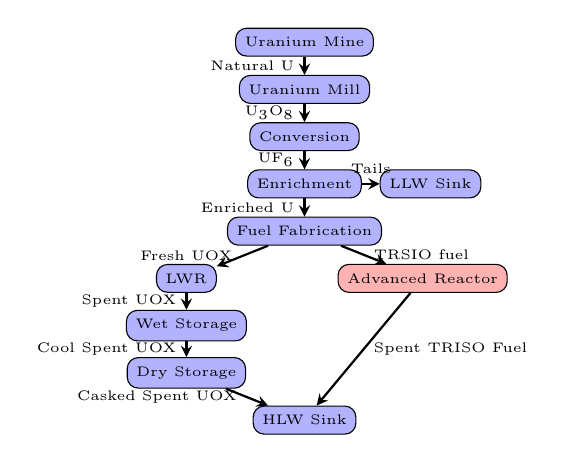
\begin{tikzpicture}[node distance=0.6cm]
            \node (mine) [agent] {\tiny Uranium Mine};
            \node (mill) [agent, below of=mine] {\tiny Uranium Mill};
            \node (conversion) [agent, below of=mill] {\tiny Conversion};
            \node (enrichment) [agent, below of=conversion]{\tiny Enrichment};
            \node (fabrication) [agent, below of=enrichment]{\tiny Fuel Fabrication};
            \node (reactor) [agent, below of=fabrication, xshift=-1.5cm]{\tiny LWR};
            \node (adv_reactor) [transition, below of=fabrication, xshift=1.5cm]{\tiny Advanced Reactor};
            \node (wetstorage) [agent, below of=reactor]{\tiny Wet Storage};
            \node (drystorage) [agent, below of=wetstorage]{\tiny Dry Storage};
            \node (sinkhlw) [agent, below of=drystorage, xshift=1.5cm]{\tiny HLW Sink};
            \node (sinkllw) [agent, right of=enrichment,xshift=1cm]{\tiny LLW Sink};
    
            \draw [arrow] (mine) -- node[anchor=east]{\tiny Natural U} (mill); 
            \draw [arrow] (mill) -- node[anchor=east]{\tiny U$_3$O$_8$}(conversion); 
            \draw [arrow] (conversion) -- node[anchor=east]{\tiny UF$_6$}(enrichment);
            \draw [arrow] (enrichment) -- node[anchor=east]{\tiny Enriched U}(fabrication);
            \draw [arrow] (enrichment) -- node[anchor=south]{\tiny Tails}(sinkllw);
            \draw [arrow] (fabrication) -- node[anchor=east]{\tiny Fresh UOX}(reactor);
            \draw [arrow] (fabrication) -- node[anchor=west]{\tiny TRSIO fuel}(adv_reactor);
            \draw [arrow] (reactor) -- node[anchor=east]{\tiny Spent UOX}(wetstorage);
            \draw [arrow] (wetstorage) -- node[anchor=east]{\tiny Cool Spent UOX}(drystorage);
            \draw [arrow] (drystorage) -- node[anchor=east]{\tiny Casked Spent UOX}(sinkhlw);
            \draw [arrow] (adv_reactor) -- node[anchor=west]{\tiny Spent TRISO Fuel}(sinkhlw);
    
            \end{tikzpicture}
        \caption{Fuel cycle facilities and material flow between facilities in the \Cyclus
        models.}
        \label{fig:fuel_cycle}
    \end{figure}
\end{columns}
\end{frame}

\begin{frame}
    \frametitle{Agent Hierarchy}
    \begin{figure}[t]
        \centering
        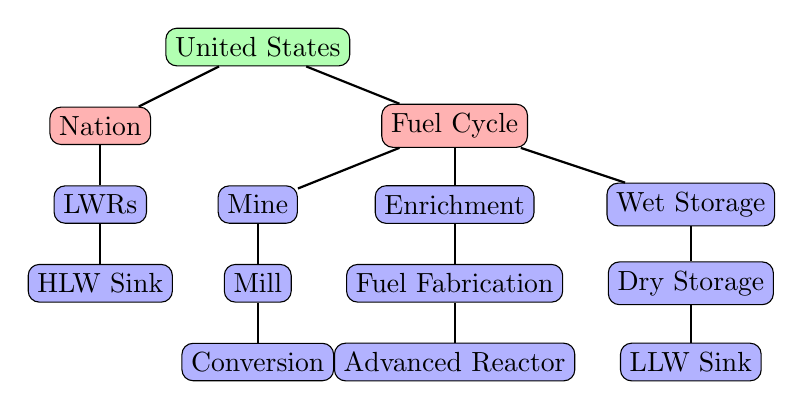
\begin{tikzpicture}[node distance=1cm]
            \node (region) [region] {United States};
            \node (inst1) [institution, below of=region, xshift=2.5cm] {Fuel Cycle};
            \node (inst2) [institution, below of=region, xshift=-2cm] {Nation};
            \node (lwr) [facility, below of=inst2] {LWRs};
            \node (mine) [facility, below of=inst1, xshift=-2.5cm] {Mine};
            \node (mill) [facility, below of=mine] {Mill};
            \node (conversion) [facility, below of=mill] {Conversion};
            \node (enrichment) [facility, below of=inst1] {Enrichment};
            \node (fuelfab) [facility, below of=enrichment] {Fuel Fabrication};
            \node (ad_rx) [facility, below of=fuelfab] {Advanced Reactor};
            \node (wet_stor) [facility, below of=inst1, xshift=3cm] {Wet Storage};
            \node (dry_stor) [facility, below of=wet_stor] {Dry Storage};
            \node (llw_sink) [facility, below of=dry_stor] {LLW Sink};
            \node (hlw_sink) [facility, below of=lwr] {HLW Sink};

            \draw [connect] (region) -- (inst1);
            \draw [connect] (region) -- (inst2);
            \draw [connect] (inst2) -- (lwr);
            \draw [connect] (inst1) -- (mine);
            \draw [connect] (fuelfab) -- (ad_rx);
            \draw [connect] (mine) -- (mill);
            \draw [connect] (mill) -- (conversion);
            \draw [connect] (inst1) -- (enrichment);
            \draw [connect] (enrichment) -- (fuelfab);
            \draw [connect] (inst1) -- (wet_stor);
            \draw [connect] (wet_stor) -- (dry_stor);
            \draw [connect] (dry_stor) -- (llw_sink);
            \draw [connect] (lwr) -- (hlw_sink);

        \end{tikzpicture}
        \caption{Oranization of agents in the simulations, green shows the region, red shows the institutions,
        and blue shows the facilities.}
        \label{fig:hierarchy}        
    \end{figure}
\end{frame}
\section{Results}
\begin{frame}
    \frametitle{Reactor Deployment}
    \begin{columns}
        \column[t]{5cm}
        \begin{itemize}
            \item The last \gls{LWR} is decommissied in 2076
            \item In the no growth scenarios (Scenarios 2 and 3) the advanced reactors are 
                  deployed starting in October 2031
            \item In the 1\% growth scenarios (Scenarios 4 and 5) the advanced reactors are 
                  deployed starting in March 2029
            \item The maximum number of advanced reactors deployed at one time 
                  in Scenarios 2-5 are 9182, 1225, 17656, and 2361 reactors, respectively
        \end{itemize}

        \column[t]{5cm}
        \vspace{-1cm}
        \begin{figure}
            \centering 
            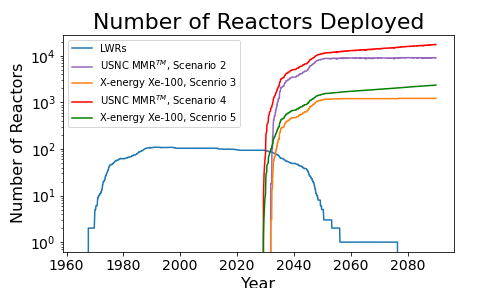
\includegraphics[scale=0.3]{figures/rxdeployment_scenarios_all.png}
            \caption{Reactor deployment schedule for \glspl{LWR} and 
            advanced reactors.}
            \label{fig:rx_deployment}
        \end{figure}
    \end{columns}
\end{frame}

\begin{frame}
    \frametitle{Energy}
    \begin{columns}
        \column[t]{5cm}
        \begin{itemize}
            \item Energy produced by \glspl{LWR} in Scenario 1 in 2025 is 91.818 GWe-y
            \item Scenarios 2 and 3 do not meet demand between 2038-2053
            \item Scenario 4 does not meet demand between 2035-2054
            \item Scenario 5 does not meet demand between 3035-2048
            \item Noticable deviations from demand in Scenarios 2, 4 when new 
                  reactors are deployed
                  secWEV;UW
        \end{itemize}

        \column[t]{5cm}
        \vspace{-1cm}
        \begin{figure}
            \centering 
            \begin{subfigure}
                \centering
                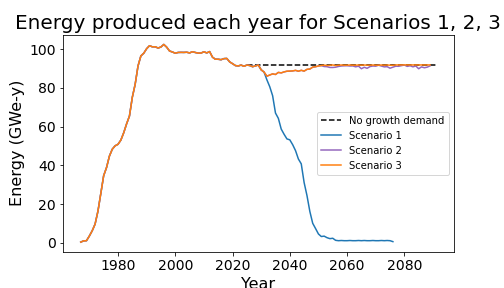
\includegraphics[scale=0.3]{figures/energy_scenarios_123.png}
                \label{fig:energy_123}
            \end{subfigure}
            \vspace{-0.8cm}
            \begin{subfigure}
                \centering
                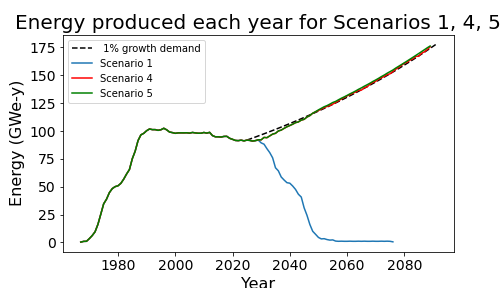
\includegraphics[scale=0.3]{figures/energy_scenarios_145.png}
                \label{fig:energy_145}
            \end{subfigure}
            \caption{Energy produced per year by all reactors in Scenarios 1-3 (top)
            and Scenarios 1, 4, 5 (bottom)}
            \label{fig:energy}
        \end{figure}
    \end{columns}
\end{frame}

\begin{frame}
    \frametitle{Uranium Mass Supply}
    \begin{columns}
        \column[t]{5cm}
            \begin{itemize}
                \item All scenarios have the same uranium demands until 
                      advanced reactors are deployed
                \item Large peaks in Scenarios 2 and 4 correspond to the 
                      deployment of new reactors
                \item Less variation with time in the uranium supplied to reactors
                      for Scenarios 3 and 5 than Scenarios 2 and 4
                \item There is a 6 month delay in when advanced reactors 
                      are deployed and fueled in Scenario 4
            \end{itemize}
        \column[t]{5cm}
        \vspace{-0.8cm}
        \begin{figure}
            \centering 
            \begin{subfigure}
                \centering
                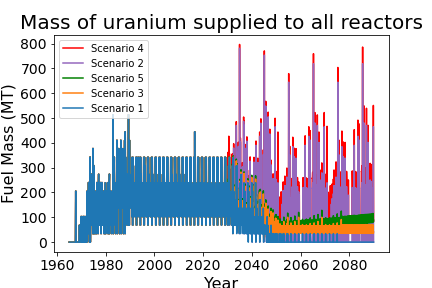
\includegraphics[scale=0.3]{figures/fuelsupply_scenarios_all.png}
                \label{fig:fuel_all}
            \end{subfigure}
            \begin{subfigure}
                \centering
                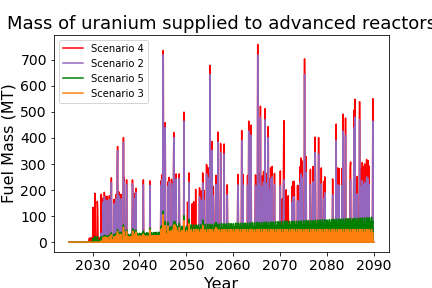
\includegraphics[scale=0.3]{figures/advancedRX_fuelsupply_scenarios_2-5.png}
                \label{fig:fuel_advancedRX}
            \end{subfigure}
            \caption{Uranium mass sent to all reactors (top)
            and only advanced reactors (bottom)}
            \label{fig:fuel}
        \end{figure}
    \end{columns}
    

\end{frame}

\begin{frame}
    \frametitle{\gls{SWU} Requirements}
    \begin{columns}
        \column[t]{5cm}
            \begin{itemize}
                \item Follows similar pattern to uranium mass 
                \item Scenarios 2 and 4 require the most \gls{SWU} 
                      because of the large mass of urnaium, despite a 
                      lower enrichment level for the advanced reactors 
                      Scenarios 3 and 5
                
            \end{itemize}
        \column[t]{5cm}
        \vspace{-1cm}
        \begin{figure}
            \centering 
            \begin{subfigure}
                \centering
                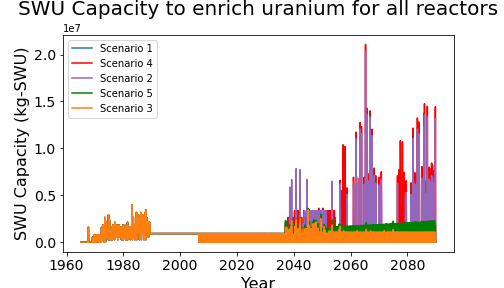
\includegraphics[height=0.35\textheight]{figures/totalswu_scenarios_all.png}
                \label{fig:swu_all}
            \end{subfigure}
            \vspace{-0.5cm}
            \begin{subfigure}
                \centering
                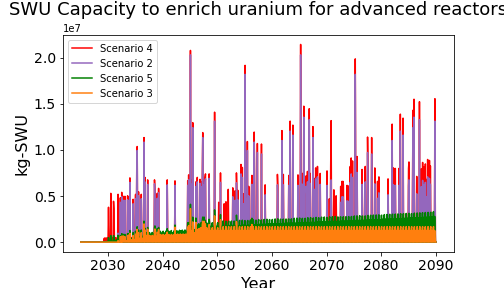
\includegraphics[height=0.35\textheight]{figures/haleuSWU_scenarios_all.png}
                \label{fig:swu_haleu}
            \end{subfigure}
            \caption{\gls{SWU} required to produce enriched uranium for all 
            reactors (top) and only advanced reactors (bottom)}
            \label{fig:swu}
        \end{figure}
    \end{columns}
    

\end{frame}


\section{Conclusions}
\begin{frame}
    \frametitle{Conclusions}
    \begin{itemize}
        \item Simulated 5 fuel cycle scenarios to investigate the material 
              requirements of deploying \gls{HALEU}-fueled reactors
        \item Transitions to the X-energy Xe-100 reactor are better able to meet 
              the energy demand of the scenarios due to longer lifetimes
        \item Transitions to the \gls{USNC} \gls{MMR}
              have significantly more material requirements than transitions to 
              the X-energy Xe-100
        \item Changing to a 1\% growth demand model requires 
              advanced reactors to be deployed 2.5 years earlier
    \end{itemize}
    \begin{block}{Ongoing Work}
        \begin{itemize}
            \item Incorporate \gls{LWR} license expiration dates
            \item Increase the amount of time in the scenario, change end date to 2125 to include 
                  replacement of X-energy Xe-100 reactors
            \item Determine how much \gls{HEU} is needed to produce the required \gls{HALEU} for 
                  each scenario
        \end{itemize}
    \end{block}
\end{frame}

\begin{frame}
    \frametitle{Acknowledgements}
    This material is based upon work supported under an Integrated University 
Program Graduate Fellowship. Any opinions, findings, conclusions, or 
recommendations expressed in this publication are those of the author(s) 
and do not necessarily reflect the views of the Department of Energy Office 
of Nuclear Energy.

Prof. Huff is supported by the Nuclear Regulatory Commission Faculty
Development Program (award NRC-HQ-84-14-G-0054 Program B), the Blue Waters
sustained-petascale computing project supported by the National Science
Foundation (awards OCI-0725070 and ACI-1238993) and the state of Illinois, the
DOE ARPA-E MEITNER Program (award DE-AR0000983), and the DOE H2@Scale Program
(Award Number: DE-EE0008832)
\end{frame}


\begin{frame}[allowframebreaks]
    \frametitle{References}
    \bibliographystyle{plain}
    {\footnotesize \bibliography{../bibliography} }
  
  \end{frame}

\end{document}
